\documentclass[11pt]{beamer}
\usepackage[spanish]{babel}
\usepackage{amsmath}
\usepackage[utf8]{inputenc}
\usepackage{amsfonts}
\usepackage{amssymb}
\usepackage{makeidx}
\usepackage{graphicx}
\usepackage{hyperref}
\usepackage{multicol}
\usepackage{float}
\usepackage{textcomp,xifthen,graphicx,color}
\usepackage{ifthen}
\usepackage{enumerate}
\usepackage{tcolorbox}
\usepackage{cprotect}
\usepackage{grffile}
\usepackage{inconsolata}
\usepackage{listings,color}
\usepackage{xcolor}
\usepackage{sansmath}
\spanishdecimal{.}
\usetheme{Dresden}
\usecolortheme{orchid}
% FONT

\usepackage{fontspec}
\setmainfont{Arial}
%\renewcommand*\familydefault{\sfdefault}

%\sffamily



%\SelectInputMappings{%
%  ntilde={ñ}
%  }

% ENVIRONMENTS
\newenvironment{m}[1]{%
	\begin{list}{}{%
			\setlength{\topsep}{0pt}%
			\setlength{\leftmargin}{#1}%
			\setlength{\listparindent}{\parindent}%
			\setlength{\itemindent}{\parindent}%
			\setlength{\parsep}{\parskip}%
		}%
		\item[]}{\end{list}}


\newenvironment{problema}[1]{%
    \par\refstepcounter{section}
	\sectionmark{#1}
    \addcontentsline{toc}{section}{Problema #1}

	\item[\textbf{{#1}.}] {}
    }

%%%%%%%%%%%%%%%%%%%%%%%%%%%%%%%%%%%%%%%%%%%%%%%%%%%%%%%%%%%%%%%%%%%%%%%
% SOME COMMANDS
\renewcommand{\baselinestretch}{1.2}
\newcommand\mynewline[1]{ \\[{#1}\baselineskip]}
\newcommand{\dem}{\begin{m}{17cm}
			$\blacksquare$
		  \end{m}}
\newcommand{\sol}{\underline{Solución}: }
\newcommand{\com}{\textbf{Comentario}: }
\newcommand\tab[1][1cm]{\hspace*{#1}}
\newcommand{\B}{\beta}
\newcommand{\cod}[1]{\texttt{\frenchspacing#1}}
\newcommand{\R}{\ensuremath{\mathbb{R}}}
\newcommand{\N}{\ensuremath{\mathbb{N}}}
\renewcommand{\labelitemii}{\ding{43}}
\newcommand{\makehigho}{\leavevmode\raise1.0ex\hbox{\tiny o}}
\newcommand\segundo{2\makehigho{ }}
\newcommand\primero{1\makehigho}
\usepackage{fancyhdr}

\makeatletter
\let\thetitle\@title
\let\theauthor\@author
\let\thedate\@date
\makeatother

% DATA

\title{Temperatura Crítica de Superconductores} % Titulo
\subtitle{Presentamos nuevos modelos} % Subtítulo
\logo{
\includegraphics[scale=0.0875]{logo-uc}}
\author{Grupo A - Estadística}		% Autor
\date{1 de Diciembre de 2020}		% Fecha
\institute[EYP2307 - Análisis de Regresión]{
	\inst{}
		Pontificia Universidad Católica de Chile \\
		Facultad de Matemáticas \\
		EYP2307 - Análisis de Regresión
        }


\AtBeginSection[]
{
	\begin{frame}<beamer>{Contenido}
		\tableofcontents[currentsection,currentsubsection]
	\end{frame}
}


\begin{document}


% PORTADA %%%%%%%%%%%%%%%%%%%%%%%%%%%%%%%%%%%%%%%%%%%%%%%%%%%%%%%%%%%%%%%%%%%%%%%%%
\begin{frame}
	\maketitle
\end{frame}

% CONTENIDO %%%%%%%%%%%%%%%%%%%%%%%%%%%%%%%%%%%%%%%%%%%%%%%%%%%%%%%%%%%%%%%%%%%%%%%
\begin{frame}[fragile]{Contenido}
	\tableofcontents
\end{frame}


% SECCION 1 %%%%%%%%%%%%%%%%%%%%%%%%%%%%%%%%%%%%%%%%%%%%%%%%%%%%%%%%%%%%%%%%%%%%%%%
\section{Avance 1}

\begin{frame}{Recursos Utilizados}
	\begin{enumerate}
		\item Usamos RStudio.
		\item R Markdown y R Sweave.
		\item GitHub.
		\item Bases de datos.
		\begin{itemize}
			\item \cod{train.csv}
			\item \cod{unique\_m.csv}
		\end{itemize}
	\end{enumerate}
\end{frame}

\begin{frame}{Objetivo Avance 1}
	\begin{itemize}
		\item Predecir la temperatura crítica de los superconductores, en base a nuestra variable respuesta \cod{critical\_temp}.
	\end{itemize}
\end{frame}

\begin{frame}{Limpieza de la base de datos}
	\begin{itemize}
		\item Como se tenían \textbf{169} variables en total, se decidió limpiar la base de datos.
		\pause
		\item Al hacer la limpieza nos quedamos solo con \textbf{34} variables.
	\end{itemize}
\end{frame}

\begin{frame}{Elección del modelo}
	\begin{itemize}
		\item Se hizo un análisis de correlación.
		\pause
		\item La variable \cod{std\_ThermalConductivity} tuvo la correlación más alta de $\mathbf{0.65}$, por lo tanto se utilizó para nuestro modelo de regresión lineal simple.
		\pause
		\item Al hacer el análisis de la varianza explicada: $R^2=\mathbf{0.43}$.
		\pause
		\item Se decidió buscar alternativas para intentar aumentar este último valor.
	\end{itemize}
\end{frame}

\begin{frame}{Buscando Alternativas}
	\begin{itemize}
		\item  Nos decidimos por un nuevo modelo.
		\pause
		\item  Utilizamos la variable \cod{range\_Valence} por ser una variable discreta y así nos quedaron \textbf{7} modelos.
		\pause
		\item  El modelo final nos quedó:
		\begin{itemize}
			\pause
			\item  $\rho = \mathbf{0.75}$.
			\pause
			\item  $R^2 = \mathbf{0.56}$.
		\end{itemize}
	\end{itemize}
\end{frame}

\begin{frame}{Objetivo del Avance 2}
	\begin{itemize}
		\item Predecir la temperatura crítica de los superconductores en base a nuestra variable respuesta, utilizando modelos de regresión lineal múltiple para mejorar los resultados obtenidos en el Avance \textbf{1}.
	\end{itemize}
\end{frame}


% SECCION 2 %%%%%%%%%%%%%%%%%%%%%%%%%%%%%%%%%%%%%%%%%%%%%%%%%%%%%%%%%%%%%%%%%%%%%%%
\section{Nuevos modelos}

\begin{frame}{Nuevos modelos}
	\begin{itemize}
		\item Creamos una serie de nuevos modelos de regresión lineal múltiple:
		\begin{enumerate}
			\item \textit{Backward}.
			\pause
			\item \textit{Forward}.
			\pause
			\item \textit{Backward-Forward}.
			\pause
			\item \cod{add1}.
			\pause
			\item \cod{drop1}.
			\pause
			\item \textit{VIF}.
			\pause
			\item Modelo con la idea del Avance \textbf{1}.
			\pause
			\item \textit{Ridge Regression}.
			\pause
			\item \textit{Lasso Regression}.
		\end{enumerate}
	\end{itemize}
\end{frame}

\begin{frame}{Nuevos modelos}
	\begin{itemize}
		\item Se utilizó la base de datos limpiada en el Avance \textbf{1} para trabajar solo con \textbf{34} variables.
	\end{itemize}
\end{frame}

\begin{frame}{Modelo con \textit{Backward}}
	\begin{itemize}
		\item Criterio AIC.
		\item Multicolinearidad $\to \mathbf{0}$ variables eliminadas.
		\item Modelo conformado finalmente por \textbf{27} variables.
	\end{itemize}
\end{frame}

\begin{frame}{Modelo con \textit{Forward}}
	\begin{itemize}
		\item Criterio AIC.
		\item Multicolinearidad $\to \mathbf{0}$ variables eliminadas.
		\item Modelo conformado finalmente por \textbf{28} variables.
	\end{itemize}
\end{frame}

\begin{frame}{Modelo con \textit{Backward-Forward}}
	\begin{itemize}
		\item Criterio AIC.
		\item Multicolinearidad $\to \mathbf{0}$ variables eliminadas.
		\item Modelo conformado finalmente por \textbf{27} variables.
	\end{itemize}
\end{frame}

\begin{frame}{Modelo con \cod{add1}}
	\begin{itemize}
		\item Criterio AIC.
		\item Multicolinearidad $\to \mathbf{0}$ variables eliminadas.
		\item Modelo conformado finalmente por \textbf{28} variables.
	\end{itemize}
\end{frame}

\begin{frame}{Modelo con \cod{drop1}}
	\begin{itemize}
		\item Criterio AIC.
		\item Multicolinearidad $\to \mathbf{0}$ variables eliminadas.
		\item Modelo conformado finalmente por \textbf{25} variables.
	\end{itemize}
\end{frame}

\begin{frame}{Modelo con \textit{VIF}}
	\begin{itemize}
		\item Se consideró el modelo conformado por todas las variables de la base de datos.
		\item Se fue eliminando el problema de multicolinearidad progresivamente.
		\item Modelo conformado finalmente por \textbf{28} variables.
	\end{itemize}
\end{frame}

\begin{frame}{Modelo con la idea del Avance \textbf{1}}
	\begin{itemize}
		\item Se crearon \textbf{7} bases de datos según \cod{range\_Valence}.
		\item Se creó un modelo para cada base de datos mediante selección \textit{Backward} con criterio AIC.
		\item Cantidad de variables:
		\begin{enumerate}
			\item Modelo para \cod{range\_Valence = 0}: \textbf{25} variables.
			\item Modelo para \cod{range\_Valence = 1}: \textbf{23} variables.
			\item Modelo para \cod{range\_Valence = 2}: \textbf{24} variables.
			\item Modelo para \cod{range\_Valence = 3}: \textbf{25} variables.
			\item Modelo para \cod{range\_Valence = 4}: \textbf{22} variables.
			\item Modelo para \cod{range\_Valence = 5}: \textbf{19} variables.
			\item Modelo para \cod{range\_Valence = 6}: \textbf{27} variables.
		\end{enumerate}
	\end{itemize}
\end{frame}

% SECCION 3 %%%%%%%%%%%%%%%%%%%%%%%%%%%%%%%%%%%%%%%%%%%%%%%%%%%%%%%%%%%%%%%%%%%%%%%
\section{Elegimos modelo}

\begin{frame}{AIC, BIC y $R^2$ de los modelos.}
		\begin{tabular}{| r | c | c | c |}
			\hline
			\textbf{Modelo} & \textbf{AIC} & \textbf{BIC} & $\mathbf{R^2}$
			\\ \hline
			\textit{Backward} & 126489.9 &  127064.9 & 0.66 \\
			\textit{Forward} & 126880.5 & 127103.5 & 0.66 \\
			\textit{Backward-Forward} & 126849.9 & 127064.9 & 0.66\\
			\cod{add1} & 126858.4 &  127081.4& 0.66\\
			\cod{drop1} & 126849.6 & 127048.7 & 0.66\\
			\textit{VIF} & 126880.5 & 127103.5 & 0.6 \\ 
			Idea Avance 1 & 121021.6 & 121840.3 & 0.74
			\\ \hline
		\end{tabular}
\end{frame}


\begin{frame}{Supuesto de \textit{Independencia}}
	\begin{itemize}
		\item Se utilizó el Test de \textit{Durbin-Watson}.
		\item Independencia de residuos $\Leftrightarrow$ Valor D entre \textbf{1.5} y \textbf{2.5}. 
		\item Ningún modelo mencionado cumple este supuesto.
	\end{itemize}
\end{frame}

\begin{frame}{Supuesto de \textit{Normalidad}}
	\begin{itemize}
		\item Se utilizó el Test de \textit{Kolmogorov-Smirnov}.
		\item Criterio: Valor-p $>0.05$.
		\item Ningún modelo mencionado cumple este supuesto.
		\item Primera solución aplicada: Transformación de \textit{Box-Cox}
		\item Segunda solución aplicada: 
	\end{itemize}
\end{frame}

\begin{frame}{Diapositiva}
	\begin{itemize}
		\item abc
	\end{itemize}
\end{frame}

\begin{frame}{Diapositiva}
	\begin{itemize}
		\item abc
	\end{itemize}
\end{frame}

\begin{frame}{Diapositiva}
	\begin{itemize}
		\item abc
	\end{itemize}
\end{frame}

\begin{frame}{Diapositiva}
	\begin{itemize}
		\item abc
	\end{itemize}
\end{frame}

\begin{frame}{Diapositiva}
	\begin{itemize}
		\item abc
	\end{itemize}
\end{frame}

\begin{frame}{Diapositiva}
	\begin{itemize}
		\item abc
	\end{itemize}
\end{frame}

\begin{frame}{Diapositiva}
	\begin{itemize}
		\item abc
	\end{itemize}
\end{frame}


% SECCION 4 %%%%%%%%%%%%%%%%%%%%%%%%%%%%%%%%%%%%%%%%%%%%%%%%%%%%%%%%%%%%%%%%%%%%%%%
\section{Ridge y Lasso Regression}

\begin{frame}{\textit{Ridge Regression}}
	\begin{itemize}
		\item \underline{Objetivo:} Minimizar \textbf{RSS}.
		\item \textcolor{blue}{\textit{Shrinkage Penalty}} : $RSS_{\text{Ridge}} = RSS_{\text{AMC}} + \textcolor{blue}{\lambda \sum^p_{j=1} \beta_j^2}$.
		\begin{itemize}
			\item $\underline{\lambda = \mathbf{0}}: RSS_{\text{Ridge}} = RSS_{\text{AMC}}$.
			\item $\underline{\lambda \geq \mathbf{0}}:$ Impacto en valores de $\B$.
			\item $\underline{\lambda \to \mathbf{\infty}}:$ $\B \to \vec{\mathbf{0}}$.
		\end{itemize}
	\end{itemize}
\end{frame}

\begin{frame}{\textit{Ridge Regression}: $\lambda$ óptimo}
	\begin{itemize}
		\item Es aquel que reduce la mayor varianza del modelo sin apenas perder ajuste.
		\item \textit{Validación cruzada}.
	\end{itemize}
\end{frame}

\begin{frame}{\textit{Ridge Regression}: Visualización}
	\begin{figure}
		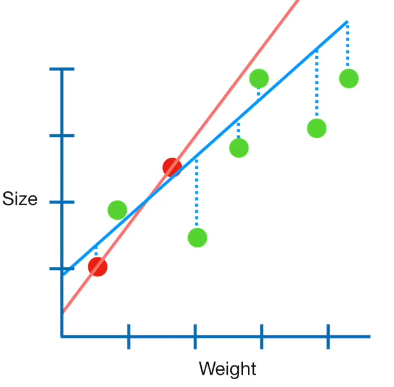
\includegraphics[scale=0.4]{figures/ridge.png}
	\end{figure}
\end{frame}


\begin{frame}{\textit{Ridge Regression}: Ventajas}
	\begin{itemize}
		\item Reduce la varianza.
		\item Datos de Entrenamiento vs. Datos de Prueba.
		\item Minimiza la influencia sobre el modelo de los predictores menos relacionados con la variable respuesta.
	\end{itemize}
\end{frame}

\begin{frame}{\textit{Ridge Regression}: Limitación}
	\begin{itemize}
		\item Modelo final incluye todos los predictores.
	\end{itemize}
\end{frame}

\begin{frame}{\textit{Lasso Regression}}
	\begin{itemize}
		\item Misma idea que en \textit{Ridge Regression}.
		\item Selección de predictores.
		\item \textcolor{blue}{\textit{Shrinkage Penalty}} : $RSS_{\text{Lasso}} = RSS_{\text{AMC}} + \textcolor{blue}{\lambda \sum^p_{j=1} |\beta_j|}$.
	\end{itemize}
\end{frame}

\begin{frame}{Comparación entre \textit{Ridge} y \textit{Lasso Regression}}
	\begin{itemize}
		\item Usamos uno u otro dependiendo del escenario.
		\item \textit{Ridge Regression}: cuando los $\B \not = \vec{\mathbf{0}}$ y tienen la misma magnitud aproximadamente.
		\item \textit{Lasso Regression}: cuando un gran grupo de parámetros $\approx \mathbf{0}$.
	\end{itemize}
\end{frame}

\begin{frame}{Resultados de la implementación en R}
	\begin{itemize}
		\item \textcolor{blue}{\textit{Ridge Regression}}:
	\end{itemize}
\end{frame}

% CONCLUSIONES %%%%%%%%%%%%%%%%%%%%%%%%%%%%%%%%%%%%%%%%%%%%%%%%%%%%%%%%%%%%%%%%%%%%
\section{Conclusiones}

\begin{frame}{Conclusiones}
	\begin{itemize}
		\item abc
	\end{itemize}
\end{frame}


% REFERENCIAS %%%%%%%%%%%%%%%%%%%%%%%%%%%%%%%%%%%%%%%%%%%%%%%%%%%%%%%%%%%%%%%%%%%%%%%
\section{Referencias bibliográficas}

\begin{frame}{Referencias bibliográficas}
	\begin{thebibliography}{10}

		\beamertemplateonlinebibitems % imagen de una URL de internet
		\bibitem{Author2019}
		https://online.stat.psu.edu/stat501/lesson/13/13.1
		\newblock{\em Weighted Least Squares}.
		\newblock{2018}

		\beamertemplateonlinebibitems % imagen de una URL de internet
		\bibitem{Author2019}
		https://rpubs.com/Joaquin\_AR/242707
		\newblock{\em Selección de predictores: Ridge y  Lasso}.
		\newblock{2016}

		\beamertemplateonlinebibitems % imagen de una URL de internet
		\bibitem{Author2019}
		https://rstatisticsblog.com/data-science-in-action/machine-learning/ridge-regression-in-r/
		\newblock{\em Simple Guide To Ridge Regression In R}.
		\newblock{2020}

		%\beamertemplatebookbibitems % imagen de revista, paper o artículo
		%\bibitem{Author19901}
		%Libro
		%\newblock{\em Autor}.
		%\newblock{2020}

	\end{thebibliography}
\end{frame}


\end{document}

